\nopagebreak
\section{theory}
\subsection{Plane parallel layer}
The investigated semiconductor samples can in first approximation be described as a plane parallel 
layer \ref{fig:fabry-perot} with a thickness $d$ and refractive index $N_2$ which acts like a fabry-perot interferometer.
\begin{figure}[h]
    \centering
    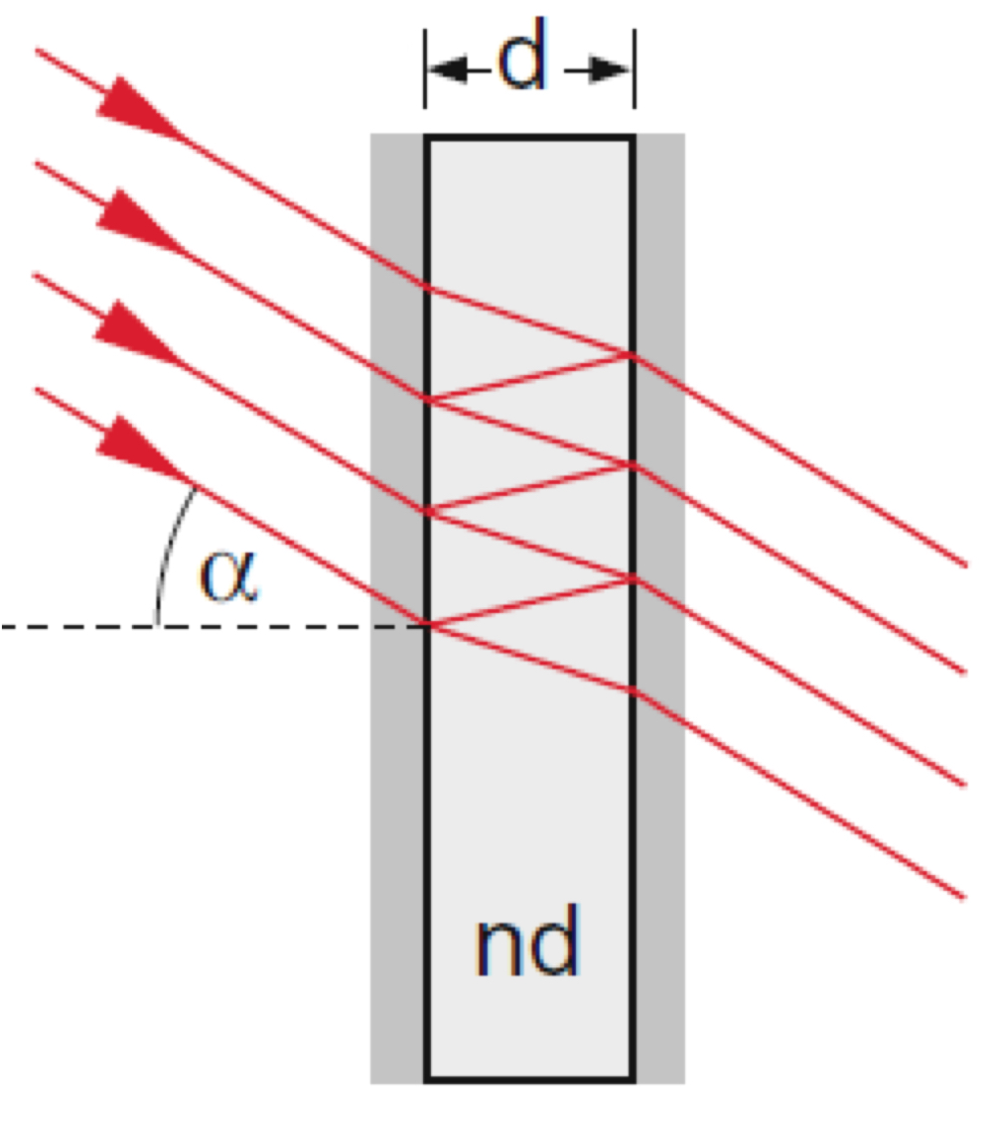
\includegraphics[width=0.3\textwidth]{Images/fabry-perot.png}
    \caption{Simplified illustration of the measured samples as a plane parallel plate
    with thickness $d$ and refractive index $N_2$. The surrounding air is described with a 
    refractive indes $N_1\approx1$ \cite{Gerthsen}}
    \label{fig:fabry-perot}
\end{figure}
Light is simpliefied as beams. Every incoming beam is partially reflected and 
partially transmittet at the first interface. The total power reflectivity $R_1$ is described with:
\begin{align}\label{eq:R1}
    R_1 = \left\lvert \frac{1 - N_2}{1 + N_2} \right\rvert^2
\end{align}
without considering the phase shift of the reflected beam. Like shown in the illustration, the total
power reflectivity of the second interface $R_2$ consists of the incoming beams and the beams reflected
at the first interface within the material. Additionally, the absorption of the material is considered.
Therefore, $R_2$ is described with:
\begin{align}\label{eq:R2}
    R_2 = R_1(1-R_1)^2 \cdot e^{-2\beta d}
\end{align}
with the absorption coefficient $\beta$ and the total power reflectivity $R_1$ of the first interface.
The assumption that the reflection of the first interface is the same as the reflection of the second
interface is in reality not correct. Disturbances like roughness of the interfaces or the absorption of the
material lead to a different reflection coeffitients of the two interfaces.\\
Considering this and the phase of the light, the total power reflectivity $R$ is described with:
\begin{align}\label{eq:R}
    R = \left\lvert \frac{(e^{i\frac{2\omega}{c}N_2d}-1)(1-N_2)}{e^{i\frac{2\omega}{c}N_2d}(1-N_2)-(1+N_2)} \right\rvert^2.
\end{align}
